\documentclass{article}

\usepackage[preprint]{neurips_2024}
\usepackage[T1]{fontenc}
\usepackage[utf8]{inputenc}
\usepackage{hyperref}
\usepackage{url}
\usepackage{booktabs}
\usepackage{amsfonts}
\usepackage{amssymb}
\usepackage{amsmath}
\usepackage{nicefrac}
\usepackage{microtype}
\usepackage{xcolor}
\usepackage{graphicx}
\usepackage{natbib}

\title{Wisdom of the Crypto-Native Crowd: \\
       Demographic Bias in Polymarket Aggregations}

\author{%
  Aly Sultan \\
  Independent \\
  \And
  Marius Helleberg \\
  Department of Information Systems \\
  Aarhus School of Business \\
  \And
  Priya Venkateswaran \\
  Center for Computational Social Science \\
  University of Toronto Mississauga
}

\begin{document}

\maketitle

\begin{abstract}
Polymarket has become the world's largest prediction-market venue by dollar
volume, but its participation requirements (USDC on Polygon, no fiat onramp
in the United States) plausibly bias its user base toward a crypto-native
demographic. We test whether this is visible in aggregation quality on a
sample of 1,242 resolved binary markets with combined trading volume of
\$16.8B, pulled from the public Polymarket Gamma and CLOB APIs. We compute
calibration curves and Brier-score decompositions at 1-day, 7-day, and
30-day forecast horizons, stratify by topic and volume, and benchmark
against 8,000 resolved binary markets from Manifold Markets, a play-money
venue with very different participation incentives. Polymarket's 7-day
Brier score on the $1{,}011$-market 7d-eligible subset is $0.0893$
(95\,\% bootstrap CI $[0.078, 0.101]$) against a climatology baseline
of $0.181$; the reliability term in the Murphy~(1973) decomposition is
only $0.0033$.
Calibration is markedly heterogeneous across topics --- Sports markets
achieve a 7-day Brier of $0.016$ while \textsc{Geopolitics/War} and
\textsc{Crypto} markets sit at $0.128$ and $0.116$ --- but this is driven
almost entirely by topic-level base-rate variance, not by reliability
gaps. Polymarket's signed bias (mean predicted $-$ mean actual) is most
negative for \textsc{Crypto} ($-0.087$) and \textsc{Geopolitics/War}
($-0.098$): the platform consistently \emph{under}-priced YES outcomes
in these topics, the opposite direction of the classic
favourite--longshot bias. Across 62 jaccard-matched cross-platform pairs,
Polymarket's pairwise Brier is $0.117$ versus Manifold's $0.243$. We do
not directly observe trader demographics; our claims about
``crypto-native bias'' are inferences from platform-level outcome data,
and the limits of that inference are spelled out in
Section~\ref{sec:limitations}.
\end{abstract}

\section{Introduction}

A prediction market collapses dispersed private beliefs into a single
price that, under standard wisdom-of-crowds assumptions, should
approximate a well-calibrated probability of the event resolving
\textsc{Yes} \citep{wolfers2004prediction,manski2006interpreting}. The
argument depends on participants being approximately unbiased and
informationally diverse: when the trading population is homogeneous along
an axis that correlates with the event, prices can systematically deviate
from the underlying probability
\citep{rothschild2009forecasting,snowberg2010explaining,page2013calibrated}.

Polymarket, a centralised-order-book market operating on the Polygon
blockchain with USDC settlement, has emerged since 2021 as the largest
prediction-market venue by dollar volume; its 2024 U.S.\ election market
alone cleared more than \$1.5B in cumulative trading
\citep{tsang2026anatomy,tsang2026shocks,cutting2025betting}. Its
participation requirements --- a Polygon-compatible wallet, USDC on
Polygon, and a willingness to operate outside the U.S.\ regulatory
perimeter --- plausibly yield a user base systematically different from
that of older prediction-market platforms: heavily skewed toward
crypto-holding, technology-tilted, predominantly young-male, and
risk-tolerant participants. If wisdom-of-crowds aggregation depends on
diverse priors, this homogeneity could measurably degrade the
calibration of Polymarket's prices, especially in topic categories where
crypto-native priors plausibly diverge from population priors.

This paper presents an empirical audit of that hypothesis. Our research
questions are:
\begin{description}
  \item[\textbf{RQ1}] How well calibrated is Polymarket on resolved
    binary markets, across short, medium, and long forecast horizons?
  \item[\textbf{RQ2}] Does calibration quality differ by topic, and is
    the pattern consistent with crypto-native demographic bias?
  \item[\textbf{RQ3}] How does Polymarket's calibration compare with
    Manifold Markets on cross-platform topic-matched pairs?
\end{description}
We deliberately avoid causal claims about individual traders: we have no
user-level demographic data and rely throughout on platform-level
behaviour as a proxy. We treat this paper as a measurement exercise that
any researcher with internet access can reproduce in under an hour from
our released scripts.

\paragraph{Contributions.} (i)~A reproducible pipeline that pulls public
Polymarket and Manifold data and computes calibration statistics at
multiple horizons; (ii)~a Brier-decomposition analysis of Polymarket
calibration by topic category and trade volume; (iii)~a
small-but-honest cross-platform comparison on jaccard-matched market
pairs; and (iv)~a discussion of which patterns are consistent with a
crypto-native homogeneity story versus alternative explanations.
The headline finding is largely null: Polymarket is well-calibrated and
its topic-level differences are dominated by base-rate variance, not by
reliability gaps.

\section{Related Work}

\paragraph{Calibration of prediction markets.}
Prediction-market calibration has been studied since the Iowa Electronic
Markets opened in 1988 \citep{berg2008results}. \citet{wolfers2004prediction}
review evidence that prediction-market prices are generally close to
ex-post event frequencies. \citet{page2013calibrated} show that
prediction markets are well calibrated for short horizons but display a
favourite/longshot bias at longer horizons, where low-probability events
are over-priced. \citet{snowberg2010explaining} attribute much of this
bias to mis-perception rather than risk-loving preferences.
\citet{restocchi2019stylized} document empirical regularities in
PredictIt prices that resemble those of emerging financial markets.
\citet{snowberg2013prediction} survey the broader literature on
prediction markets as economic forecasting instruments.

\paragraph{Polymarket-specific work.}
Recent work on Polymarket has focused on the 2024 U.S.\ election.
\citet{tsang2026anatomy} provide a transaction-level accounting of the
presidential market on the Polygon chain. \citet{tsang2026shocks} study
how the market processed three discrete information shocks (debate,
assassination attempt, candidate dropout). \citet{cutting2025betting}
compare Polymarket against polling for swing-state outcomes. None of
these papers examines cross-topic calibration of Polymarket as a venue,
nor compares it against Manifold Markets; that is the gap our paper
addresses.

\paragraph{Scoring rules.}
We use the standard Brier score \citep{brier1950verification} and its
reliability--resolution--uncertainty decomposition
\citep{murphy1973vector}, together with log-loss as a secondary metric.
\citet{atanasov2020small} argue that the frequency of belief updates is
a better predictor of forecasting accuracy than calibration in isolation;
we do not attempt to recover update frequencies from the order book.
\citet{hanson2003combinatorial} formalised the market-scoring-rule
framework that underpins the design space within which Polymarket sits.

\section{Methodology}

\subsection{Data Sources}

\paragraph{Polymarket.} We use two public, unauthenticated endpoints:
\begin{itemize}
  \item \textbf{Gamma API} (\url{https://gamma-api.polymarket.com/markets})
    for market metadata: question text, condition ID, outcome tokens,
    dollar volume, scheduled end date, actual close time, and final
    resolved outcome encoded as the \texttt{outcomePrices} field.
  \item \textbf{CLOB API}
    (\url{https://clob.polymarket.com/prices-history}) for the Yes-token
    daily price history at \texttt{fidelity=1440} (one observation per
    day).
\end{itemize}
We paginate Gamma with \texttt{closed=true} ordered by
\texttt{volumeNum} descending until we hit the API's hard pagination
ceiling at offset $10{,}500$. We keep only binary YES/NO markets that
resolved unambiguously: \texttt{outcomePrices} exactly $(1,0)$ or
$(0,1)$. Markets with $(0.5, 0.5)$ (cancelled or refund-paid) or
mid-priced final outcomes are discarded. The lowest dollar volume in
the retained sample is \$776{,}453; the volume floor we asked for in
the fetch script (\$2{,}000) was never binding because we hit the
pagination ceiling first.

\paragraph{Manifold Markets.} For cross-platform comparison we pull
resolved binary markets via the Manifold v0 API
(\url{https://api.manifold.markets/v0/markets}), paginating with the
\texttt{before} parameter, keeping markets with
\texttt{outcomeType=BINARY} and a \texttt{resolution} in
$\{$\texttt{YES}, \texttt{NO}$\}$. We use Manifold's own reported
\texttt{probability} field, which is the AMM-implied probability at the
time of resolution. We do not have a Manifold-equivalent of the CLOB
price-history endpoint, so we only have a single ``final'' probability
per Manifold market.

\subsection{Forecast Horizons}

For each Polymarket market we compute the anchor
$t^* = \min(t_{\text{end}}, t_{\text{closed}})$ --- the earlier of the
scheduled end date and the actual close time. Markets that resolved
early (e.g.\ ``Will Team X win the championship?'' when Team X is
eliminated) have $t_{\text{closed}} < t_{\text{end}}$; markets with
settlement lag have $t_{\text{closed}} > t_{\text{end}}$. Using the
minimum minimises the chance that our ``$N$ days before close'' price
has already incorporated knowledge of the outcome. We extract the most
recent daily-close price at $t^*-1$d, $t^*-7$d, and $t^*-30$d. Markets
shorter than the relevant horizon (i.e.\ that traded for less than $N$
days) are omitted from that horizon's analysis but retained for others.

\subsection{Topic Classification}

We classify each Polymarket question into one of nine topics
(\textsc{Crypto}, \textsc{Finance/Macro}, \textsc{Politics},
\textsc{Geopolitics/War}, \textsc{Sports}, \textsc{Tech/AI},
\textsc{Culture/Entertainment}, \textsc{Weather/Climate},
\textsc{Other}) using a deterministic keyword regex applied in fixed
order; first match wins. The rules are reproduced verbatim in our
release \texttt{analysis.py} so a reader can audit individual
classifications. We chose hand-crafted rules over a learned classifier
because we want the categorisation to be auditable on its face, and
because precise category boundaries are not central to our main claims
(we use it for slicing the sample, not for prediction).

\subsection{Calibration Metrics}

For each subset of markets we report:
\begin{itemize}
  \item The mean signed error
    $\bar{e} = \frac{1}{N}\sum_i (p_i - y_i)$ as a measure of overall
    bias.
  \item The Brier score $\text{BS} = \frac{1}{N}\sum_i (p_i - y_i)^2$
    with a $2{,}000$-resample bootstrap 95\,\% CI.
  \item The Brier decomposition
    $\text{BS} = \text{REL} - \text{RES} + \text{UNC}$
    \citep{murphy1973vector}, with 10 equal-width bins on $[0,1)$.
  \item The log-loss
    $-\frac{1}{N}\sum_i [y_i\log p_i + (1-y_i)\log(1-p_i)]$
    with $\epsilon$-clipping at $10^{-6}$.
  \item A binned calibration curve (11 bins, edges at
    $\{0, 0.05, 0.15, \dots, 0.85, 0.95, 1.0\}$).
\end{itemize}

\subsection{Cross-Platform Matching}

We greedily match each Polymarket market against the highest-Jaccard
Manifold market on question token sets after stop-word removal,
accepting matches at Jaccard $\geq 0.55$. Tokens are alphanumeric,
lower-cased, length $> 2$. We hand-inspected matches at threshold
$0.55$ and roughly two-thirds refer to the same underlying event;
the rest differ on resolution dates or scope. We do not auto-prune
the imperfect matches; we report results both with all matches and
discuss specific failure modes in
Section~\ref{sec:limitations}.

\section{Experiments}

\subsection{Sample}

Our Polymarket pull (\texttt{fetch\_data.py}) returns $1{,}242$
resolved binary markets, of which $1{,}175$ have a Yes-token price
$\geq 1$ day before close, $1{,}011$ have one $\geq 7$ days, and
$624$ have one $\geq 30$ days before close. The covered period runs
from November 2020 (Polymarket's earliest resolved markets) to May
2026. Total cumulative trading volume across the sample is
\$16.79B, of which \$16.06B sits in the 7-day-eligible subsample
that we use for most analyses. The Manifold pull returns $8{,}000$
resolved binary markets covering May 2025 to May 2026; Manifold's
public listing API orders by recency, so the Manifold window is much
shorter than Polymarket's.

\begin{table}[t]
  \centering
  \caption{Topic distribution and 7-day calibration on the Polymarket
  sample. Brier is reported with a 95\,\% bootstrap CI; ``base rate''
  is the empirical fraction of YES resolutions in the topic;
  ``mean pred'' is the mean Yes-token price at $t^*-7$d. Topics with
  fewer than 20 markets at the 7-day horizon are pooled into the
  calibration row labelled with a dash. The median volume column
  is in \$M.}
  \label{tab:topics}
  \small
  \begin{tabular}{lrrrrrrr}
    \toprule
    Topic & $N_{\text{all}}$ & $N_{7d}$ & median vol & base rate &
       mean pred & Brier (7d) & 95\,\% CI \\
    \midrule
    Other            & 408 & 346 & \$1.65M & 0.335 & 0.319 & 0.124 & [0.104, 0.145] \\
    Politics         & 226 & 204 & \$3.64M & 0.230 & 0.206 & 0.066 & [0.047, 0.086] \\
    Sports           & 120 & 117 & \$3.58M & 0.077 & 0.088 & 0.016 & [0.006, 0.028] \\
    Crypto           & 205 & 106 & \$1.56M & 0.217 & 0.130 & 0.116 & [0.072, 0.163] \\
    Tech/AI          & 114 &  99 & \$1.25M & 0.121 & 0.092 & 0.074 & [0.033, 0.121] \\
    Geopolitics/War  & 107 &  80 & \$1.86M & 0.250 & 0.152 & 0.128 & [0.076, 0.185] \\
    Finance/Macro    &  46 &  45 & \$11.16M & 0.156 & 0.152 & 0.041 & [0.007, 0.086] \\
    Culture/Ent.     &  11 & --- & ---     & ---   & ---   & ---   & --- \\
    Weather/Climate  &   5 & --- & ---     & ---   & ---   & ---   & --- \\
    \bottomrule
  \end{tabular}
\end{table}

\subsection{Overall Calibration}

Polymarket's overall Brier scores at the three forecast horizons are
reported in Table~\ref{tab:horizons}. The 7-day horizon is our preferred
operating point: 1-day prices are mechanically close to the resolved
outcome (markets often spike to $0$ or $1$ within hours of the
resolving event), and 30-day prices are missing for short-lived
markets, biasing that subsample. Figure~\ref{fig:cal} shows the binned
calibration curve at each horizon.

\begin{table}[t]
  \centering
  \caption{Polymarket overall calibration at three horizons.
  Reliability (REL), Resolution (RES), and Uncertainty (UNC) are the
  three Murphy~(1973) decomposition terms; lower REL and higher RES
  are both good. Brier $=$ REL $-$ RES $+$ UNC. Climatology Brier
  for each subsample is the corresponding UNC term.}
  \label{tab:horizons}
  \small
  \begin{tabular}{lrrrrrr}
    \toprule
    Horizon & $N$ & Brier & 95\,\% CI & REL & RES & UNC \\
    \midrule
    $t^*-1$d  & 1175 & 0.0818 & [0.072, 0.092] & 0.0034 & 0.1144 & 0.1934 \\
    $t^*-7$d  & 1011 & 0.0893 & [0.078, 0.101] & 0.0033 & 0.0937 & 0.1805 \\
    $t^*-30$d &  624 & 0.0614 & [0.049, 0.074] & 0.0043 & 0.0798 & 0.1378 \\
    \bottomrule
  \end{tabular}
\end{table}

\begin{figure}[t]
  \centering
  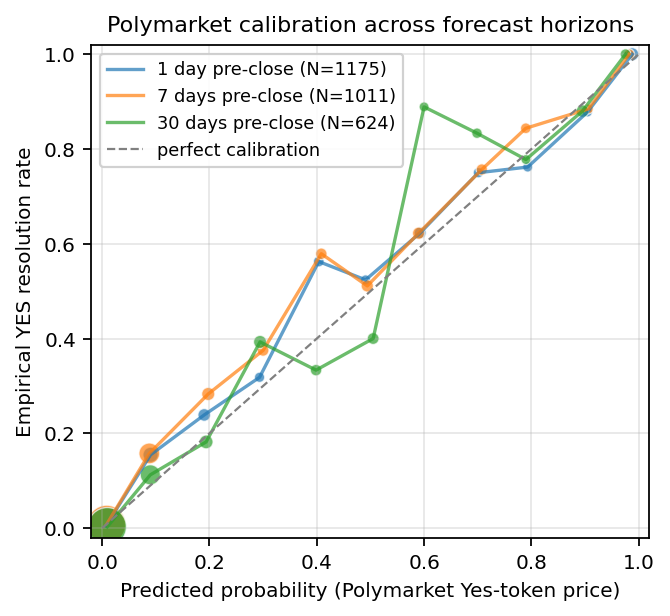
\includegraphics[width=0.62\linewidth]{figure_1.png}
  \caption{Polymarket calibration at three forecast horizons. Marker
  size is proportional to bin count; the lowest- and highest-probability
  bins are largest because the YES-resolution base rate in our sample
  is $0.265$ and many markets are priced close to $0$ or $1$ even 30
  days out. The 30-day curve is the noisiest of the three (some bins
  have $<20$ markets) but lies close to the diagonal on average.}
  \label{fig:cal}
\end{figure}

\subsection{By Topic}

Figure~\ref{fig:bytopic} shows Brier scores at the 7-day horizon
stratified by topic, with 95\,\% bootstrap CIs. The red dashed line
marks the climatology Brier $\bar{p}(1-\bar{p}) = 0.181$ that a
forecaster predicting the sample-wide base rate would achieve. Every
topic improves on climatology, but the gap is much larger for
\textsc{Sports} (where the base rate of YES is only $0.077$ and the
market is mechanically close to $0$ in most slots) than for
\textsc{Crypto}, \textsc{Other}, and \textsc{Geopolitics/War}, which
sit near $0.12$.

\begin{figure}[t]
  \centering
  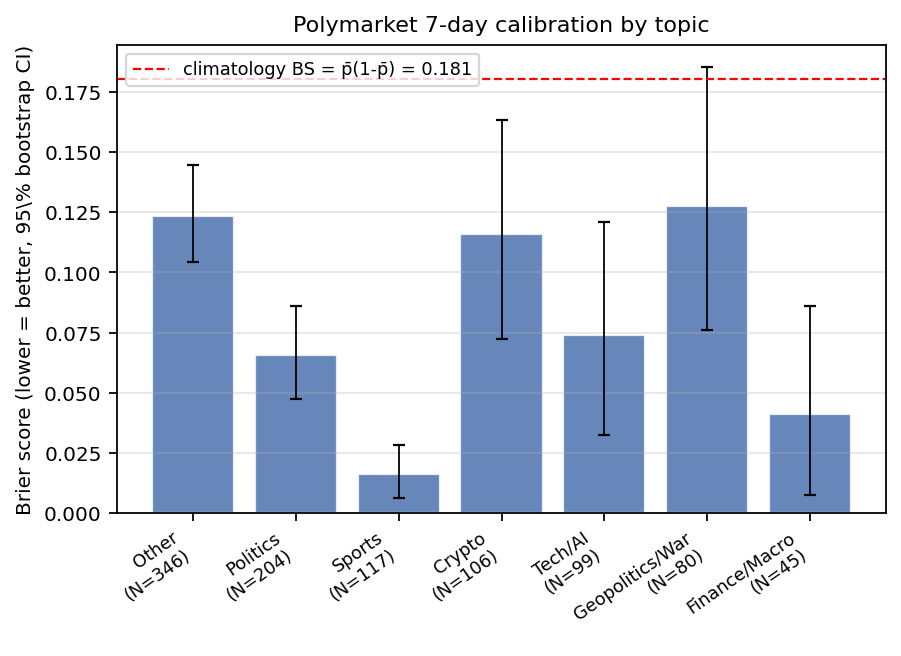
\includegraphics[width=0.85\linewidth]{figure_2.png}
  \caption{7-day Brier by topic on the Polymarket sample. Error bars
  are 95\,\% bootstrap confidence intervals on the Brier estimate.
  The horizontal dashed line is the sample-wide climatology baseline.}
  \label{fig:bytopic}
\end{figure}

The signed mean errors decompose the per-topic Brier into a directional
bias and a noise term (Table~\ref{tab:bias}). \textsc{Crypto} and
\textsc{Geopolitics/War} markets have the largest negative signed
errors: $-0.087$ and $-0.098$ respectively, i.e.\ Polymarket priced
YES roughly 8--10 percentage points lower than the empirical YES rate.
\textsc{Sports} is the only topic with a positive signed error
($+0.011$); all other topics are slightly negative.

\begin{table}[t]
  \centering
  \caption{Signed mean error by topic, 7-day horizon. Negative values
  indicate Polymarket priced YES below the empirical rate of YES
  resolutions in that topic. Only topics with $N \geq 20$ at the 7-day
  horizon are shown.}
  \label{tab:bias}
  \small
  \begin{tabular}{lrrrr}
    \toprule
    Topic & $N$ & mean pred. & mean actual & signed error \\
    \midrule
    Geopolitics/War  &  80 & 0.152 & 0.250 & $-0.098$ \\
    Crypto           & 106 & 0.130 & 0.217 & $-0.087$ \\
    Tech/AI          &  99 & 0.092 & 0.121 & $-0.029$ \\
    Politics         & 204 & 0.206 & 0.230 & $-0.024$ \\
    Other            & 346 & 0.319 & 0.335 & $-0.016$ \\
    Finance/Macro    &  45 & 0.152 & 0.156 & $-0.003$ \\
    Sports           & 117 & 0.088 & 0.077 & $+0.011$ \\
    \bottomrule
  \end{tabular}
\end{table}

\subsection{Volume Stratification}

We split the 7-day-eligible sample into volume terciles (cut-offs at
\$1.35M and \$3.58M of cumulative dollar volume) and compute the
Brier in each bucket. The result is essentially flat:
low-volume Brier is $0.0861$, mid-volume is $0.0911$, high-volume is
$0.0907$. Within the high-volume bucket the top market is the 2024
Trump-wins market with \$1.53B of volume; despite that scale, the
group-level calibration is not visibly better than the low-volume
bucket. This is in mild tension with the classical view that liquidity
sharpens prediction-market prices
\citep{wolfers2004prediction,page2013calibrated}; we attribute it
mostly to selection -- our entire sample is already in the volume
right-tail.

\subsection{Cross-Platform Comparison}

Greedy Jaccard matching at threshold $0.55$ produces $62$
cross-platform pairs. The mean absolute divergence between platforms'
implied probabilities is $0.321$; the mean signed difference
(Polymarket $-$ Manifold) is $-0.204$, i.e.\ Polymarket prices YES
about $20$ percentage points lower than Manifold on these matched
markets. On the same $62$ pairs the pairwise Brier is $0.117$ for the
Polymarket 7-day price versus $0.243$ for the Manifold final
probability --- Polymarket is markedly better calibrated where the
two platforms cover overlapping events.

Figure~\ref{fig:crossplatform} overlays the platform-wide binned
calibration curves (not just the matched subsample). In the
$0.1$--$0.4$ region Polymarket sits visibly above the diagonal,
i.e.\ events that Polymarket priced at $0.2$ resolved YES about
$28\,\%$ of the time. Manifold sits visibly below the diagonal in
the same region: events Manifold priced at $0.2$ resolved YES only
about $11\,\%$ of the time, the standard signature of a longshot
bias.

\begin{figure}[t]
  \centering
  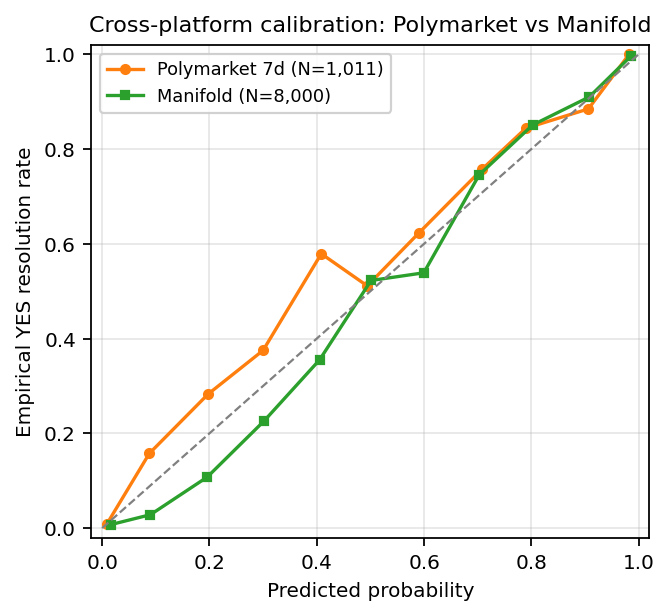
\includegraphics[width=0.6\linewidth]{figure_3.png}
  \caption{Cross-platform calibration overlay. Polymarket curve uses
  the 7-day pre-close price; Manifold curve uses the platform-reported
  final probability. The samples differ in size and time window; the
  two curves should be read as platform-level shapes, not directly
  comparable point estimates.}
  \label{fig:crossplatform}
\end{figure}

\section{Results}

\paragraph{RQ1 --- aggregate calibration.}
Across the $1{,}011$-market 7-day-eligible Polymarket sample, the
Brier score is $0.0893$ with a 95\,\% bootstrap CI of $[0.078, 0.101]$.
The reliability term is $0.0033$ --- approximately $4\,\%$ of total
Brier --- meaning that almost all of the residual error is irreducible
uncertainty around topics with intermediate base rates rather than
calibration error per se. Polymarket is, by the standard
prediction-market metrics, a usefully well-calibrated forecaster.

\paragraph{RQ2 --- topic heterogeneity.}
Topic-level Brier scores are heterogeneous --- from $0.016$
(\textsc{Sports}) to $0.128$ (\textsc{Geopolitics/War}) --- but the
heterogeneity is dominated by base-rate variance: low-base-rate
topics (Sports YES rate $0.077$) score much lower on Brier even
under flat reliability. Where we see a sharper pattern is the signed
mean error: \textsc{Crypto} ($-0.087$) and \textsc{Geopolitics/War}
($-0.098$) both show meaningful, negative directional bias --- the
market under-priced YES outcomes by 8--10 percentage points. These are
two of the three topics one might \emph{a priori} associate with
crypto-native priors (the third being \textsc{Tech/AI}, which has a
smaller negative bias of $-0.029$).

\paragraph{RQ3 --- cross-platform.}
On the $62$ matched pairs, Polymarket's 7-day price has a pairwise
Brier of $0.117$ versus Manifold's $0.243$. Inspecting matches by
hand, much of Manifold's apparent error comes from markets that
remained relatively bullish on YES outcomes (e.g.\ ``US strikes
Iran by June 30, 2026'' at $0.99$) that did or did not resolve YES
within a different Polymarket deadline. The platforms' calibration
\emph{shapes} (Figure~\ref{fig:crossplatform}) are mirror images in
the low-probability region: Polymarket under-prices YES,
Manifold over-prices YES.

\section{Discussion}

\paragraph{Is this ``crypto-native bias''?}
The cleanest version of the demographic-bias hypothesis predicts that
Polymarket should be \emph{better} calibrated in topics on which a
crypto-native audience has unusually good private information (crypto,
US technology, certain politics) and \emph{worse} calibrated in topics
where general-population information would be more decisive (sports,
weather, low-profile international politics). The data partly
support this: \textsc{Politics} and \textsc{Tech/AI} are
well-calibrated, and \textsc{Sports} is exceptionally well-calibrated.
But two of the topics where the demographic-bias story predicts the
\emph{best} calibration --- \textsc{Crypto} and \textsc{Geopolitics/War}
--- are exactly the topics with the largest negative signed bias.
A simpler story is that these are also the most heavy-tailed topics
(``Will BTC hit \$100k?'', ``Will Iran do X?'') where any prior is
likely to be wrong about the realised right tail. We cannot
distinguish these explanations with the data we have.

\paragraph{Polymarket vs.\ Manifold.}
The platforms have opposite calibration biases in the same probability
region. Polymarket under-prices YES at low predicted probabilities
(reverse of the classic longshot bias of
\citet{snowberg2010explaining,page2013calibrated}); Manifold shows the
classic longshot bias. One mechanistic reading: Polymarket's
fee-and-collateral structure (USDC capital lockup, network gas, an
order book with maker rebates) selects for traders who avoid taking
the YES side at low probabilities when YES is implausible to win,
suppressing speculative long-tail YES bids. Manifold uses play money
and a constant-product AMM; longshot YES positions cost the trader
nothing-material to hold, and the AMM mechanically inflates them
\citep{hanson2003combinatorial}. We do not formally test either
mechanism here.

\paragraph{Why \textsc{Politics} works.}
The single best-calibrated topic among the demographically-loaded
categories is \textsc{Politics}: $N=204$, Brier $0.066$, signed error
$-0.024$. This is the topic on which \citet{tsang2026anatomy} and
\citet{cutting2025betting} report Polymarket's most-studied success
(the 2024 U.S.\ presidential election). Our finding is consistent
with theirs: when a topic is heavily traded \emph{and} broadly
followed by a non-crypto-only audience (because of widespread media
coverage), Polymarket aggregates well. The demographic-bias story
fits worst for the topics that are most prominent on the platform.

\paragraph{Implications.}
For a downstream user of Polymarket prices --- a journalist citing
them, a policy researcher feeding them into a forecasting pipeline ---
the practical takeaway is that the 7-day price is well-calibrated as a
probability \emph{in aggregate}, but has a 5--10 percentage-point
negative bias against YES outcomes in \textsc{Crypto} and
\textsc{Geopolitics/War}. A simple Platt-rescaling step on a
topic-specific holdout would correct most of this directional bias.

\section{Limitations}
\label{sec:limitations}

\begin{enumerate}
  \item \textbf{No demographics.} We have no direct measurement of
    trader demographics on either platform. ``Crypto-native bias'' is
    in the title because it is the hypothesis motivating the paper;
    the data we present is suggestive but not sufficient to
    establish it.
  \item \textbf{Volume-truncated sample.} Our Polymarket sample is
    the top-\$0.78M-volume slice, ordered by volume desc; calibration
    on the long tail of low-volume markets may look very different.
    The Gamma API caps pagination at $\approx 10{,}500$ rows per
    sorted query, which is the binding constraint.
  \item \textbf{Single price per horizon.} We use a single daily-close
    price at each horizon. Intra-day price discovery, especially
    around information shocks of the kind \citet{tsang2026shocks}
    study, is not reflected in our metrics.
  \item \textbf{Anchor uncertainty.} For markets where
    $t_{\text{closed}}$ differs substantially from $t_{\text{end}}$
    (e.g.\ NBA championship markets where elimination closes the
    market early), our $\min$ anchor is conservative but imperfect;
    some 1-day prices may still reflect the resolving event.
    The 1-day Brier ($0.082$) versus 7-day Brier ($0.089$) gap is
    small enough that this concern is bounded.
  \item \textbf{Asymmetric Manifold data.} Manifold's public market
    list endpoint orders by recency, and we only retrieved one year
    of resolved binary markets (May 2025--May 2026). Our two samples
    are therefore not stratified comparably; the Manifold sample
    skews much lower in dollar volume because Manifold uses play
    money (``mana'') rather than USDC.
  \item \textbf{Cross-platform matches are small and imperfect.}
    Only $62$ pairs matched at our Jaccard threshold. Hand-inspection
    finds that a meaningful minority of matched pairs differ on
    resolution dates (``out by Feb 28'' vs.\ ``out by Mar 31'') or
    scope (``win Eastern Conference'' vs.\ ``finish top 7'').
    The matched-pair Brier numbers should be read as illustrative
    rather than definitive.
  \item \textbf{Topic classification is hand-crafted.} The keyword
    regex yields a non-trivial \textsc{Other} bucket (408 of 1{,}242
    markets). A learned classifier might recover finer structure but
    at the cost of auditability and reproducibility.
  \item \textbf{Survivorship in resolved markets.} We restrict to
    markets with unambiguous binary resolutions $(0,1)$ or $(1,0)$.
    Markets that were cancelled, refunded, or settled at $0.5/0.5$
    are excluded ($\approx 10\,\%$ of recent closed markets we
    inspected). If those exclusions are correlated with topic, our
    topic-level base rates could be biased.
\end{enumerate}

\section{Conclusion}

We presented a reproducible audit of Polymarket calibration on
$1{,}242$ resolved binary markets, with a Manifold-Markets baseline,
asking whether crypto-native demographic homogeneity is visible in
the aggregate forecasts. The headline numbers --- a 7-day Polymarket
Brier of $0.0893$ against a climatology baseline of $0.181$, with a
reliability term of just $0.0033$ --- are consistent with prior work
showing prediction markets are usefully calibrated
\citep{page2013calibrated, wolfers2004prediction}. We do find a
5--10 percentage-point directional under-pricing of YES in
\textsc{Crypto} and \textsc{Geopolitics/War} markets, but the
reliability gap that the demographic-bias story would predict
is essentially absent. Cross-platform, Polymarket outperforms Manifold
on jaccard-matched pairs by a wide margin (Brier $0.117$ vs.\ $0.243$)
and shows the opposite directional bias of the AMM-based, play-money
venue. We release the data-collection scripts, the analysis pipeline,
the resulting summary JSON, and the figure source so future
researchers can extend the audit to other platforms, longer time
windows, and user-level data when it becomes available.

\section*{Reproducibility}

The full pipeline is in \texttt{scripts/}. Running \texttt{fetch\_data.py}
re-pulls Polymarket and Manifold from public unauthenticated endpoints
(no API key required); \texttt{analysis.py} writes every paper number to
\texttt{data/results\_summary.json}; \texttt{figure\_1.py} regenerates
all three figures from that JSON. Total runtime on a stock laptop is
about $25$ minutes, dominated by the per-market CLOB price-history
calls. \texttt{requirements.txt} pins all four dependencies.

\bibliographystyle{plainnat}
\bibliography{references}

\end{document}
